%!TEX program = xelatex
\documentclass[10pt, compress, handout]{beamer}
\usetheme[titleprogressbar]{m}

\usepackage{booktabs}
\usepackage[scale=2]{ccicons}
\usepackage{minted}

\usepgfplotslibrary{dateplot}

\usemintedstyle{trac}

\setbeamertemplate{caption}[numbered]
\setbeamertemplate{theorems}[numbered]
\newtheorem{crl}{Corollary}[theorem]
\newtheorem*{solution*}{Solution}

\usepackage{algorithm}
\usepackage[noend]{algpseudocode}

\usepackage{version}
%\excludeversion{proof}
%\excludeversion{solution*}

\usepackage{mathtools}
\usepackage{multicol}
\usepackage{qtree}

\makeatletter
\def\old@comma{,}
\catcode`\,=13
\def,{%
	\ifmmode%
	\old@comma\discretionary{}{}{}%
	\else%
	\old@comma%
	\fi%
}
\makeatother

\title{CSCI 3190 Tutorial of Week 12}
\subtitle{Longest Common Subsequence}
\author{LI Haocheng}
\institute{Department of Computer Science and Engineering}

\begin{document}

\maketitle

\begin{frame}[allowframebreaks]
	\frametitle{Tree}
	\begin{example}
		\begin{enumerate}[(a)]
			\item Show that the sum of the degrees of the vertices of a tree with $n$ vertices is $2n-2$.
			\item For $n \ge 2$, let $d_1, d_2, \cdots , d_n$ be $n$ positive integers such that $d_1 + d_2 + \cdots + d_n = 2n -2$. Show that there
			exists a tree whose vertices have degrees $d_1, d_2, \cdots, d_n$. 
		\end{enumerate}
	\end{example}
	\newpage
	\begin{proof}
		\begin{enumerate}[(a)]
			\item A $n$-vertex tree has $n-1$ edges so that the total degree is $2n - 2$.
			\item For $n = 2$, this is trivial. Suppose $\forall$ positive $d_i$ such that $\Sigma_{i = 1}^{n - 1} d_i = 2n - 4$, $\exists$ a tree $T^\prime$ whose vertices have degrees $d_1, d_2, \cdots, d_{n - 1}$. Then $\forall$ positive $d_i$ such that $\Sigma_{i = 1}^{n} d_i = 2n - 2$, since $d_i$ cannot be all greater than 1 or less than 2, without loss of generality, let $d_{n - 1} > 1, d_n = 1$. Hence we can remove $d_n$ and subtract $d_{n - 1}$ by 1 so that $\Sigma_{i = 1}^{n - 1} d_i = 2n - 4$ and we can find a tree $T^\prime$. After that we can add vertex $d_n$ as a leaf of $d_{n - 1}$ to build the final tree $T$.
		\end{enumerate}
	\end{proof}
\end{frame}

\begin{frame}[fragile]
	\frametitle{Traversal}
	\begin{columns}
		\begin{column}{.5\linewidth}
			\onslide<1->\begin{example}
				Construct a DFS and a BFS traversal for the graphs in Figure starting with node B as the root.
			\end{example}
			\onslide<2>\begin{solution*}
				\begin{enumerate}[(a)]
					\item \begin{description}
						\item[DFS] B, A, C, F, D, E
						\item[BFS] B, A, C, D, E, F
					\end{description}
					\item \begin{description}
						\item[DFS] B, A, D, E, C
						\item[BFS] B, A, C, D, E
					\end{description}
				\end{enumerate}
			\end{solution*}
		\end{column}
		\onslide<1->\begin{column}{.5\linewidth}
			\begin{figure}
				\centering
				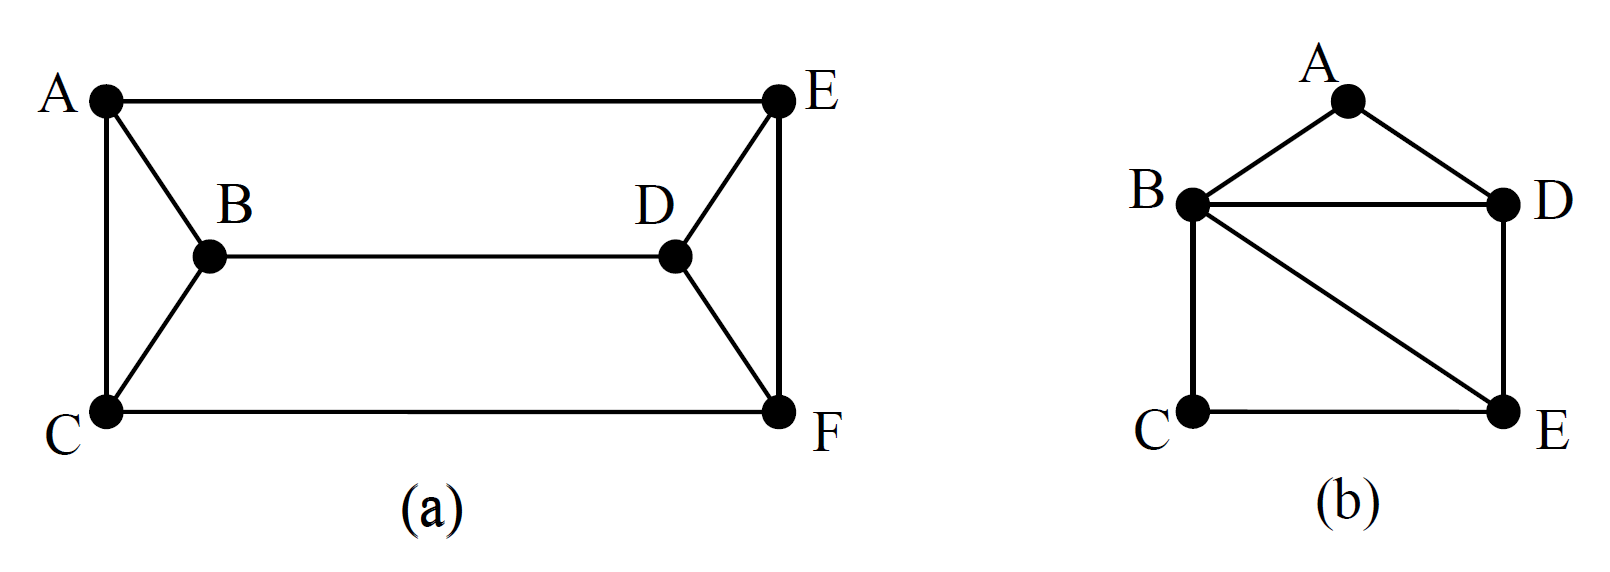
\includegraphics[width=\linewidth]{fg-1}
			\end{figure}
		\end{column}
	\end{columns}
\end{frame}

\plain{Questions?}

\end{document}
